\section{Installazione}
Sia per utilizzare l’applicazione web che per utilizzare l'app mobile è necessario seguire i seguenti step:
\begin{enumerate}
    \item Clonare il repository
    \item Avviare il server e-commerce
\end{enumerate}

Successivamente in base al prodotto che vogliamo utilizzare ci saranno dei passaggi diversi, ossia:

\begin{itemize}
    \item Avvio server webApp
    \item Avvio app mobile
\end{itemize}

\subsection{Clonazione repository}
La clonazione del repository può avvenire in due modi:
\begin{enumerate}
    \item Scaricare direttamente il codice in formato.zip\\
    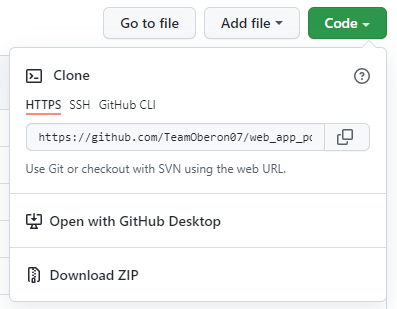
\includegraphics[scale = 0.5]{img/githubclone.PNG}
    \item Clonare il repository usando il comando su un terminale:\\
    git clone \href{https://github.com/TeamOberon07/web_app_poc.git}{https://github.com/TeamOberon07/repoDelProdotto}
    
    \item accedere alla cartella dov'è stato scaricato il prodotto
\end{enumerate}
\subsection{Avvio server e-commerce}
Per avviare il server che simula l'e-commerce:

\begin{enumerate}
    \item aprire un terminale nella cartella dove è presente mock\_e-commerce (repository diverso da quello della webApp)
    \item usare il comando: npm install (primo avvio)
    \item usare il comando: npm run server (questo utilizzerà il comando: npx json-server --watch ./src/e-comm\_db.json --port 8000)
\end{enumerate}

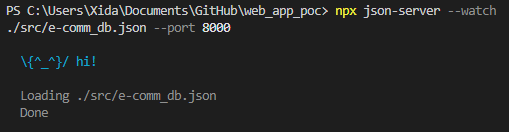
\includegraphics[]{img/ecommerce.PNG}

\subsection{Avvio server webApp}
Per avviare la webApp:
\begin{enumerate}
    \item aprire un terminale nella cartella dove è presente la webApp
    \item usare il comando: npm install (primo avvio)
    \item usare il comando: npm start
    \item si aprirà automaticamente una pagina nel browser predefinito dove visualizzare la webApp \\
    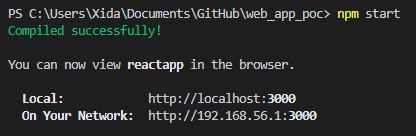
\includegraphics[]{img/webApp.PNG}
\end{enumerate}
Per creare una build ottimizzata per la produzione usare i seguenti comandi:
\begin{enumerate}
    \item npm run build
    \item npm install -g serve (se non è stato già installato)
    \item serve -s build
\end{enumerate}

\subsection{Avvio mobile app}
Per utilizzare l'applicazione mobile è necessario:

DA COMPLETARE